\documentclass[11pt]{article}

%------------ PACKAGES ----------
\usepackage{mathtools}
\usepackage{csquotes}
\usepackage{graphicx}
\usepackage{titling}
\usepackage{float}
\usepackage{csvsimple}
\graphicspath{ {./figures/}}
\newcommand{\bigO}{\mathcal{O}}
\renewcommand*{\thefootnote}{(\arabic{footnote})}

%------------ MARGINS ----------
\addtolength{\oddsidemargin}{-.75in}
\addtolength{\evensidemargin}{-.75in}
\addtolength{\textwidth}{1.5in}
\addtolength{\topmargin}{-.75in}
\addtolength{\textheight}{1.5in}

%------------ START DOCUMENT ----------
\begin{document}

%------------ TITLE INFO ------------
\begin{titlingpage}
    \centering\par
    {\huge University of Birmingham\par}
    {\small School of Computer Science\par}
        \vspace{0.8cm}
    {\Large Final Year Project\par}
        \vspace{0.8cm}
    {\Huge\bfseries Portfolio Optimization Using Geometric Mean, Risk Correlation 
        \& Multi-Objective Genetic Algorithms\par}
        \vspace{1.7cm}
    {\Large Alex Lewis\par}
    {\large 1638326 \par}
        \vspace{1cm}
    {\tiny Supervised by\par}
    {\Large Shan He\par}
        \vspace{0.7cm}
    {\large \today \par}
        \vspace{0.3cm}
        \hrulefill
        \vspace{0.3cm}
    \begin{abstract}
            \vspace{0.1cm}
            In modern portfolio theory an optimal portfolio is one which balances
            risk and reward. An efficient portfolio is one which lies along the
            edge of portfolios which cannot physically have higher return without
            increased risk. Portfolio optimization is the process of finding these
            efficient portfolios, and it's crucial from an investment standpoint
            so that an informed decision can be made as to how risky a portfolio
            is compared to its predicted return. An under explored area is risk
            evaluation. It is normally done using the Mean-Variance model, or
            value at risk. I propose a novel technique to find the correlation
            of assets inside a portfolio, and associating some mathematical
            value to this correlation. This set of calculations was applied
            from every asset to find the riskiness of a portfolio. Combining
            this with the classic return prediction of the geometric mean creates
            a multi-objective problem. This can then be efficiently solved
            using the latest iteration of genetic algorithms - NSGA-II.
            This more computer science oriented approach aims to tackle portfolio
            optimization from a new angle. The resulting approach ended up
            under-performing compared to more simple portfolios, but the new
            approach to risk showed promise. The portfolios produced had much reduced
            variance, as well as providing a level of user control to more accurately
            select how risky to make their portfolios, while maintaining an efficient
            portfolio. With further work on the usage of risk correlation, portfolios
            could be much improved by optimizing for this objective and hopefully
            a return to match other portfolio creation methods.
    \end{abstract}
\end{titlingpage}

\tableofcontents
\pagebreak

\section{Introduction To Portfolio Optimization}

    A portfolio is a collection of economic assets, and the optimization of such an
    entity is the process of maximizing its return over time, while minimizing the
    risk of the collection.

    More specifically, in the case of this project, the assets we are analyzing are
    stocks. Whereas in the more general case, a portfolio would consist of choosing
    assets over multiple markets of completely different types, such as: the price of 
    materials, currencies, bonds, etc.

    A lot of work is already based on this simple premise of min-maxing - risk and
    reward. It was first discussed by Harry Markowitz in 1952 \cite{Markowitz}
    in his famous paper. He talks about the geometry of the Risk Reward space
    of portfolio's in an abstract way. Thus creating the concept of the efficient frontier.
    This was developed further into more specific, and more mathematically implementable
    forms: Value at Risk \cite{ValueAtRisk, Ghaoui}, Mean Variance Model (named
    after Markowitz's paper) \cite{Robert, SidWard} and many, many more.
    The full review of all these other optimization solutions is best left
    to economists. To gloss over the details, and to reach a summary: portfolio
    optimization is a classical and important problem in economics, which has
    been studied in great detail. It's been studied because it's such a useful
    problem to solve as one would like to
    not waste time investing in a low risk/low reward portfolio if the same
    effect could be achieved using risk-free investments. Compounding
    that with the fact that a higher risk/higher return portfolio could
    be more desirable. Modern portfolio theory is about finding the ``efficient
    frontier" of portfolios which are the spectrum of portfolios ranging from
    high risk to low risk. Then an individual investor can choose a portfolio
    from this frontier based on how willing they are to a accept a level of
    risk.

    The focus of this project is to use the incredibly hard computable nature
    of this problem, and solve it with insight from computer science. The focus
    is not to fully solve portfolio optimization, but rather taking the problems
    presented in these various papers and proceeding to formulate an experiment to test
    whether using genetic algorithms comes to good solutions, namely: finding portfolios on the
    `efficient frontier'. More technically,
    the application of risk correlation with multi-objective genetic algorithms
    to find the ``efficient frontier" of portfolios. From those portfolios a choice
    would be given to an investor.

\subsection{Portfolio Optimization History \& Assumptions}

    Kelly Criterion \cite{Kelly} is a great theoretical achievement. Such a simple formula so
    perfectly describes how to play a system in order to gain the most from it. In fact
    it completely solves how to invest into a single stock. But alas
    stocks and trades are themselves not a repeatable and positive mathematical expectation
    game. Hence why we need to adapt the equations so that we can try to apply them to the
    real world, and deal with more than one stock.

    A big assumption which is being made from now on, by other papers about portfolio
    optimization - sometimes implicitly,
    is that we can model a stock as a random variable. It
    implies, from past data, that we can construct a model which will be able
    to predict the probabilities associated with different outcomes of future events.
    This differs from a normal random variable in a few key ways. A random variable in
    mathematics once defined will always act the same. Whereas a stock will
    depend upon its past data to define its functionality, and hence is not fixed to act
    the same.

    Furthermore this means that as we gain new data, our model is constantly shifting.
    We do not have a fixed way to tell us probabilities of all future outcomes.
    To top this, we made another assumption: that it's feasible to use past data to predict
    future events.

    This line of thinking has been criticized by the famous book ``A Random Walk Down
    Wall Street" by Burton Malkiel \cite{BurtonMalkiel}. It uses
    key economic historical events and many studies to describe how investing and trading are
    a futile game, compared to compound interest or using an Index like S\&P 500. This is
    simply a summation of the top 500 stocks in the US stock market.

    Instead of applying mathematics and statistics to your stock purchasing, the book
    suggests that this is contrary to the 
    very nature of randomness. Humans look for patterns in all things. True 
    randomness seems to be against the very nature of what it is to be human, which is why
    there is still contention as to the ideas in the book. The book reaches a conclusion that
    if you examine stock prices in a given period you can always find an arbitrary
    system that would produce a positive return for that period.

    A system which will always work and produce a positive return, and be mathematically sound
    (i.e. it will work infinitely) is an impossibility. We do not have an infinite amount of
    time to test our systems on infinite data.

    However, as much as I like the argument presented in the book and the complete contrast to
    the statistically minded way to analyze stocks, buying a stock of an
    actual business is valued on how the business provides a product or service.
    Looking back at businesses it becomes easier to see how the value of its stock is directly
    related to the people in it, the manning of the ship.

    For me, the only way to reason to myself that statistics and analysis are still 
    useful follows this train of thought: a market is a system of people.
    To predict this system accurately would require knowledge of every individual's
    thought process. Once the system can have accurate predictions made about its
    future, it is possible to perfectly predict the outcome of every stock. Then
    we simply invest in the highest performing stock - at zero risk. However, this
    dream scenario seems so improbable that we have to try a different approach
    all together
    \footnote{A system of people is something I don't believe we will ever fully understand.
    Since it would require us to have full understanding of how the brain functions. Which
    is almost certainly beyond the scope of this project}.

    Instead of looking at the causes of stock value. i.e. the people, we can try to look
    at the just the value of the stock and infer from that which stocks are more
    likely to continue similar behaviour. This 
    statistical and short term analysis can give us insights as to 
    how it might work. Rather than determining the cause and effect, we just use the effect
    to try and predict future effects.

    One does not need to understand gravity to predict a river running downhill. Merely
    enough exposure to any kind of river will show the same effect, all rivers you
    encounter will run downhill. The fact that you don't understand the cause of rivers
    running downhill is unimportant to the prediction that all
    rivers run downhill. Obviously this metaphor is not perfect, but it is in the
    same vein as portfolio optimization, understanding the causes of stock price changes
    would be far more helpful. As understanding gravity is a far deeper and more useful
    insight than the act of predicting rivers running downhill. Because gravity, confirms
    that you will \textit{never} see a river running uphill. Therefore in the same
    essence: understanding a stock price change requires understanding the force behind
    it's change, or understanding the stock prices gravity equivalent. Alas, there is
    currently no gravity equivalent for stock prices.

\subsection{Portfolio Optimization History Continued: Optimal \(f\)}

    \begin{displayquote}[Ralph Vince \cite{Ralph}] \textit {
        For any given independent trials situation where you have an edge (i.e. positive 
        expectation) there exists an optimal fixed
        fraction (f) between 0 and 1 as a divisor of your biggest loss to bet on each event.
    } \end{displayquote}

    As it turns out this optimal \(f\) is similar to what Kelly describes in his paper. 
    And as Ralph proceeds, he explains how Kelly criterion is a perfect solution for 
    fixed size gambles with fixed wins and losses.

    But then the book reaches a different conclusion. It goes on to state that for any system where 
    the win or loss is always changing {(like the stock market)}, the Kelly formula does find
    the correct optimal \(f\).
    So instead the book proposes finding the optimal \(f\) by instead using the geometric
    mean. The geometric mean models the reinvestment technique over a series of trades.
    The most optimal system to reinvest into will have a higher geometric mean than a
    worse system. \emph{Aside: We can use the estimated geometric mean because it is
    basically the same, while being computationally less expensive}:

    \begin{equation}\label{eq:TWR}
        TWR = \displaystyle\prod^{N}_{i=1}1 + f \times \frac{- trade_i}{biggest loss}
    \end{equation}
    \begin{equation}\label{eq:GeoMean}
        Geometric Mean = exp(\frac{1}{N} \times Ln(TWR))
    \end{equation}

    where:
    \begin{flalign*}
    f &= \text{The optimal } f &&\\
    N &= \text{The number of trades} &&\\
    trade_i &= \text{The profit loss of the } i^{th} \text{ trade from the set of trades} &&\\
    biggest loss &= \text{The biggest loss from the set of trades} &&\\
    exp(x) &= \text{The exponential function} &&\\
    Ln(x) &= \text{The natural logarithm function} &&
    \end{flalign*}

    Equation from Ralph Vince's book\cite{Ralph}.
    To maximize our profit from a set of trades we want to optimize for the highest possible 
    geometric mean. Since \(f\) is a free standing variable which cannot be made the subject 
    of the equation, we can only use iteration to find a good estimate.


\subsection{Portfolios Compared to Single Stocks}

    It's a classical way of thinking to also consider diversification
    of your investments. Intuition tells us a single stock with a calculated optimal \(f\) that predicts
    good results may still have ``unlucky streaks" in which you can run out of money before
    your luck turns. This concept is intuitive, \textit{``Don't put all your eggs in
    one basket"}, otherwise our problem would be solved. By using Kelly's
    formula \cite{Kelly} we find the return of each stock individually, choose
    the highest stock and our portfolio is simply that stock.

    \begin{equation}\label{eq:Kelly}
        f = \frac{(b \times p - (1 - p))}{b}
    \end{equation}

    where:
    \begin{flalign*}
        f &= \text{The best size as a fraction of your portfolio} &&\\
        b &= \text{The net odds on the wager. i.e. your win } b + \text{ wager staked} &&\\
        p &= \text{The probability of winning} &&
    \end{flalign*}

    Therefore we want a way to reduce our \(f\) by the correct amount
    to account for large streaks. Additionally we use the left over unused money to invest in
    another (ideally uncorrelated) stock.
    This complicates the problem of finding optimal \(f\)s for a set of stocks greatly.
    An \(f\) for each stock needs to be found which best grows that specific stock, while
    also considering the chance of that stocks failure, creating a balancing act of
    risk versus reward over the entire set of \(f\)s.

    Thinking of the optimal \(f\) as a single point, inside a space of trades/bets. When we have 
    only a single trade/bet, we are doing calculations in a 2D space, and we have a line which 
    represents our optimal \(f\). However as the number of trades/bets increases we gain
    another dimension for each one.

    Therefore a single \(f\) would lie on a line; a set of \(f\)s with 2 stocks lies on a
    plane; a set of \(f\)s with 3 stocks lies on a 3D object; a set of \(f\)s with 4 stocks
    lies on a 4D object; and
    etc. The \(f\) suddenly becomes a multi variable coordinate which must be 
    exactly correct. If a single axis is out then you can miss the hill of positive 
    growth, even if every other axis lined up. This means we need to define a new function
    to find the individual \(f\)s for all the bets,
    but with relation to each other. We cannot compute each optimal \(f\) for every stock
    independently.


\subsection{Risk - A New Interpretation}

    Linking back to Kelly Criterion, the riskiness of a random variable is accounted for.
    When using Kelly's formula, equation \ref{eq:Kelly} needs no further calculations
    to account for how risky the variable is. And this is also true of geometric mean growth
    for stocks. The geometric mean accounts for the variance in the data of a single stock, as the
    equations \ref{eq:TWR} \& \ref{eq:GeoMean} are accounting for risk implicitly.

    But we need a new calculation to find the risk of the portfolio. And furthermore we would
    like a way to correlate stocks together so that we can more wisely spread our money.

\subsubsection{Mathematical Definition}

    Given the motivation from our the above sections, we would now like to formally define our
    evaluation function for how well a portfolio performs given a set of \(f\)s. Which describes
    how we spread our money over a set of stocks.

    \begin{equation}\label{eq:G}
        G(f_1...f_m) = \left( \displaystyle\prod^{m}_{k=1} HPR_k \right) ^{ \left( \displaystyle\frac{1}{\sum^{m}_{k=1}Prob_k} \right)}
    \end{equation}
    \begin{equation}\label{eq:HPR_k}
        HPR_k = \left( 1 +  \displaystyle\sum^{n}_{i=1} f_k \times \frac{- PL_{k,i}}{BL_k} \right) ^{Prob_k}
    \end{equation}
    \begin{equation}\label{eq:Prob_k}
        Prob_k = \left( \displaystyle\prod^{n - 1}_{i=1} P(i_k | j_k)\right)^{\frac{1}{n - 1}}
    \end{equation}

    where:
    \begin{flalign*}
    n &= \text{The number of trades or bets in the } k^{th}\text{set} &&\\
    m &= \text{The number of stocks} &&\\
    f_k &= \text{The optimal } f \text{ for that }k^{th} \text{ set, where } f > 0 &&\\
    PL_{k,i} &= \text{The outcome for the } i^{th} \text{ trade or bet associated with the } 
        k^{th} \text{ set} &&\\
    BL_k &= \text{The worst trade or bet for the } k^{th} \text{ set} &&\\
    P(i_k | j_k) &= \text{Roughly it is the risk of }i^{th} 
        \text{ trade or bet associated with the } k^{th} \text{ set given the risk of the } &&\\
        & j^{th} \text{ trade or bet associated with the } k^{th} 
        \text{ set. Which is easy to calculate for coins, but I will explain} &&\\
        & \text{later how it is calculated for actual stocks} &&
    \end{flalign*}

    This equation is also from Ralph's Book \cite{Ralph} which is an excellent starting point,
    but it needs to be adapted to include this idea of correlation among stocks. And furthermore
    it needs to be decoupled, so that the risk of the overall portfolio is also found. The motivation
    for such a thing is because we would like to be able to create a range of portfolios with
    differing levels of risk and reward, thus allowing a choice inside this range.


\subsubsection{Calculating Risk} \label{section:CalcR}

    Here we are actually constructing the risk calculation for a stock in a more concrete form.
    So we must operate under some assumptions and natural patterns of a stock. 

    Proposed Model of a Stock: 
    \begin{itemize}
        \item{Open {\&} Close values for a given arbitrary time period}
        \item{A ratio of correlation to other stocks}
        \item{Holes of Open {\&} Close values may occur}
    \end{itemize}

    Calculating the profit/loss of a stock at time period is now trivial and useful.
    Renaming the change in value at each time period \(i\) to \(PL_i\) we can find
    statistical facts about the stock.

    \begin{align}
        \text{mean: }
            \mu &= \frac{\sum^{n}_{i=1} PL_i}{n} \label{eq:StockMean} \\
        \text{variance: } 
            \sigma^2 &= \frac{\sum^{n}_{i=1} (PL_i - \overline{PL})^2}{n} \label{eq:StockVar}
    \end{align}

    where:
    \begin{flalign*}
    n &= \text{The number of trades for a given time period in the stock } PL &&\\
    PL_n  &= \text{The result of trading the stock on the } n^{th} \text{ trade} &&\\
    \overline{PL} &= \text{The mean of the stock } PL \text{ as calculated by equation \ref{eq:StockMean}} \\
    \end{flalign*}


    Using this data we can transform a stock into a distribution which we can use to estimate
    the likelihood of the next \(PL_i\) being above a certain value. In our case we transform
    the normal distribution using equations \ref{eq:StockMean} and \ref{eq:StockVar} to find
    the mean and variance of the stock, and hence change the normal distribution. Then it is
    simple enough to use tables to find probabilities we want. It should be noted that the
    assumption that a stock is a normal distribution has sizable implications. It ties into
    our original assumption that stocks can be modeled as random variables.

    \begin{equation} \label{eq:StockProb}
        P (PL) = \big( PL \sim \Phi(\mu, \sigma^2) \big) < 0
    \end{equation}

    where:
    \begin{flalign*}
    PL \sim \Phi (\mu, \sigma^2) &= \text{The cumulative normal distribution, adjusted to the mean } \mu \text{ and variance } \sigma^2 &&\\
    \text{ of the stock } PL\\
    \end{flalign*}

    Since calculating \(\Phi (\mu, \sigma^2)\) is incredibly hard and
    a perfect value isn't critical, we can settle for using tables as a close enough
    estimate.

    Currently two frequent problems are overlooked if we were to implement any risk
    function: `holes' in the data and older data becoming less relevant as time goes on.
    To account for those problems a change to the implementation is that we specify a time
    period and a range of time to
    take data from. This has multiple advantages, the first one being that we can choose to
    use only the most recent data about a stock. Secondly it builds directly into the algorithm,
    the fact that the calculation will not use all available data from a stock, hence dealing
    with `holes' at the same time. \textbf{Note:} This change to the algorithm does
    not directly affect the actual equation, but the implementation specifically, hence
    no reference will be made to `skipping' data in the equations succeeding.

    Now for the more complex part of the risk calculation. While the algorithm for it is
    simple, finding the data for it is a hard problem in itself. The equation
    \(P(i_k | j_k)\) (from equation \ref{eq:Prob_k}) hides the details behind the \(|\) symbol.
    Normally in statistics
    the probability of \(P(X | Y)\) means `The probability of \(X\) given \(Y\) has occurred'
    which in a normal probability space is actually just a shorthand for:

    \begin{equation*}
        P ( X | Y ) = \frac{P(X \cap Y)}{P(Y)}
    \end{equation*}

    But in our stock based world we don't have an equivalent function \(\cap\) and hence
    we don't have the function \(|\) as well. The best we can do is assume that \(\cap\)
    is roughly equivalent to multiplying together the two stocks in question, and then
    assuming that \(\div\) is roughly equivalent to multiplying that by some amount of
    correlation. We cannot just multiply and divide as if they are independent probabilities as
    the first stock will just cancel out, hence doing nothing. So our function becomes:

    \begin{equation*}
        P ( X | Y ) = P ( X ) \times P ( Y ) \times C_{X, Y}
    \end{equation*}

    where:
    \begin{flalign*}
    C_{X, Y} &= \text{The pre-calculated correlation of stock } X \text{ to stock } Y&&\\
    P( X ) &= \text{The probability of } X \text{ given by the equation \ref{eq:StockProb}} \\
    \end{flalign*}

    However this doesn't work for lots of stocks as each probability is a smaller value than 1.
    Hence when these probabilities are multiplied all together, the value gets ever smaller
    regardless of if each chance was
    actually quite high. For example, say we had 25 stocks, and each stock has a 0.9
    chance to make money, and for simplicity each correlation to every stock is 0.8. We would
    expect the chance for a single stock correlated with other stocks to also be high, but:

    \begin{flalign*}
        \text{for all stocks } P &= 0.9 \times 0.9 \times 0.8 &&\\
        \text{hence } P &= 0.648 ^ {25} &&\\
        P &= 0.00001947041 \\
    \end{flalign*}

    So even in this example, with really high odds, the overall chance will be incredibly low.
    Therefore we need to use something which both preserves
    the chances of every stock, while taking into account how correlated something is.
    This is also important later as you will see why the correlation of all stocks matters
    in equation \ref{eq:DecoupleR}.

    The solution is to use a weighted average over the stocks.
    In the case where the correlation is negative we simply do \(1 - P(PL)\)
    when we calculate the average.

    \begin{equation} \label{eq:StockWeight}
        P ( X | Y ) = 
        \begin{cases}
            \displaystyle\frac 
                {P( X ) + (P ( Y ) \times C_{X, Y})}
                {1 + C_{X, Y}} 
                & \text{ if } C_{X, Y} >= 0\\
            \\
            \displaystyle\frac
                {P( X ) + ((1 - P ( Y )) \times - C_{X, Y})}
                {1 - C_{X, Y}} 
                & \text{ if } C_{X, Y} < 0
        \end{cases}
    \end{equation}

    This is our final equation to find \(P(i_k | j_k)\) (from equation \ref{eq:Prob_k})
    as it has the behaviour we need considering all the other constraints that are needed.

    Back to the claim that the algorithm is simple - all we do is find a
    weighted average of the stocks based on how correlated they are. At a conceptual level
    this is relatively simple. But, the complexity comes from how to find, and calculate,
    good values for the table \(C\). Some non-perfect solutions are:

    % TODO WILL
    \begin{enumerate}
        \item{Calculating the actual correlation: either Spearman's, or some other mathematical technique}
        \item{Using some form of NLP (Natural Language Processing) to figure out how related the stocks are in the real world}
        \item{Grouping stocks by which industry they are in and assigning each group a correlation}
        \item{Assuming all stocks are independent}
        \item{Some other way of correlating stocks I haven't considered}
        \item{Or a combination of all the above}\label{item:C}
    \end{enumerate}

    The answer to the question ``how to find a good \(C\)?" is probably worth its own paper, since
    its almost definitely point \ref{item:C}. Which requires a more complex analysis of the systems
    that make up a stock. At the end of the day the numbers we can gather about a stock never
    tell the full story. A stock is a part of a business, and a business is simply a is a
    group of people working together to sell a product or service to other people.
    Using numbers to analyze how people will succeed in selling
    a product or service will always come up short compared to knowing and understanding
    the people who are ultimately doing the selling.

    For the sake of simplicity, because this is a proof of concept, we will calculate the
    correlation as it's mathematically defined.
    For example calculating the correlation between 2 stocks \(PL_1\) and \(PL_2\) is
    done as so:

    \begin{align}
        C_{PL_1, PL_2} = 
        \frac{
            \displaystyle\sum^{n}_{i=1} (PL_{1, i} - \overline {PL_1})(PL_{2, i} - \overline {PL_2})
        }{
            \sqrt{
                \displaystyle\sum^{n}_{i=1}(PL_{1,i} - \overline {PL_1})^2 
                \displaystyle\sum^{n}_{i=1}(PL_{2,i} - \overline {PL_2})^2
            }
        }
        \label{eq:Correlation}
    \end{align}

\section{Decoupling \(G\)} \label{section:DecoupleG}

    In the original equations \ref{eq:G}, \ref{eq:HPR_k}, and \ref{eq:Prob_k}.
    \(G\) is coupled with the risk of the portfolio
    by raising the inner calculation to 1 over the sum of all risks for every stock.
    There is another approach, which is to keep the two equations separate and use multi-
    objective genetic algorithms to solve it. The motivation for this is to balance risk
    and reward independently, contrasting to the original \(G\) which lowers the gain
    by coupling it with the risk exponentially. We would also gain a Pareto set of
    optimal portfolio's to choose from, if one was more risk averse then you could choose
    a less risky portfolio from the set.

    \begin{equation}\label{eq:DecoupleG}
        G(f_1...f_n) = \displaystyle\prod^{m}_{k=1} \left(
                1 + \displaystyle\sum^{n}_{i=1} f_k \times \Big(
                    \frac{- PL_{k,i} }{BL_k}
                \Big)
            \right)
    \end{equation}

    \begin{equation}\label{eq:DecoupleR}
        R(f_1...f_n) = \displaystyle\prod^{m}_{k=1} \left(
                1 + f_k \times \Big(
                    \forall y \in m \to P(k|y)
                \Big)
            \right)
    \end{equation}

    where:
    \begin{flalign*}
    n &= \text{The number of trades or bets in the } k^{th}\text{ set} &&\\
    m &= \text{The number of stocks} &&\\
    f_k &= \text{The optimal } f \text{ for that } k^{th} \text{ set, where } f > 0 &&\\
    PL_{k,i} &= \text{The outcome for the } i^{th} 
        \text{ trade or bet associated with the } k^{th} \text{ set} &&\\
    BL_k &= \text{The worst trade or bet for the } k^{th} \text{ set} &&\\
    P(k|y) &= \text{Equation \ref{eq:StockWeight} with the stock } k \text{ correlated 
    with every other stock in the set } m &&
    \end{flalign*}

\subsection{Inspiration and Novelty?}

    Now we can use these functions separately to evaluate both risk and reward of the
    portfolio. You get a Pareto Set \cite{Kaisa} - A non dominated efficient frontier. From
    which a choice of risk vs reward can then be made
    by a human. To the best of my current knowledge, equation \ref{eq:DecoupleR} is a new
    way of thinking about the risk of the portfolio.
    Section \ref{section:CalcR} reaches a conclusion which I believe to be
    unique. However, Ralph's work \cite{Ralph} is what inspired this line of thought
    and furthermore it is the basis of my work for equation \ref{eq:DecoupleR}, as well as
    the aggregate for equation \ref{eq:DecoupleG}.

    It was the most natural mathematical solution, given our stocks can not be fully modeled
    as a random variable. Estimating the chance of success using a normal distribution
    adjusted to a stocks value, gives insight into the stock, which is useful for calculating
    a risk value for something which is inherently hard to quantify. The number calculated
    will never be a perfect representation of the risk, but can be a helpful indicator.

\section{Solving \(f\) with respect to \(G\) and \(R\)}

    Solving the decoupled equations \ref{eq:DecoupleG} \& \ref{eq:DecoupleR} for the highest
    value of \(G\) and lowest value of \(R\) will give the best return on our portfolio
    given the current data.
    Intuition would suggest some form of iteration to check every combination of \(f\) to find
    the best performing \(f\) is a good first solution. This has two major problems.
    The first problem with this solution is that for every stock we add to our portfolio, 
    we gain fractorially many more combinations to check.

    \begin{equation*}
        \text{Number of combinations to check for: } (f_1...f_m) = m!
    \end{equation*}

    Which in some scenarios may be feasible, but because of our second major problem, the computation
    time of our evaluation functions, it becomes completely impossible to actually calculate
    the mathematically correct solution in the lifetime of the universe.
    What follows is the Big \(\bigO\) calculation for equations \ref{eq:DecoupleG} \&
    \ref{eq:DecoupleR}:

    \begin{equation*}
        \text{Decoupled: } \bigO (
            m! \times (n^m + (nm)^m)
        )
    \end{equation*}

    where:
    \begin{flalign*}
    n &= \text{The number of trades or bets in the stock} &&\\
    m &= \text{The number of stocks} &&
    \end{flalign*}

    The decoupled equation grow
    in number of calculations incredibly quickly, in fact too quickly to ever be
    solved by a pure mathematical solution. So we end up with an equation we want
    to solve, with no mathematically helpful properties (differentiable being
    the most important) to be able to do a either a heuristic, a regression
    or a gradient based approach.


\subsection{Genetic Algorithms}\label{section:GA}

    \begin{displayquote}[Albert Bethke \cite{Bethke}] \textit {
        To find the point at which a real-valued function takes it maximal value ...
        If you don't know of any special properties of the function, then you
        should use a method which is more general like genetic algorithms.
    } \end{displayquote}

    Genetic algorithms (GA), first 
    discussed by John Holland \cite{Holland} in 1975, then developed by so many
    others, such as Melanie Mitchell, Kalyanmoy Deb, and Albert Bethke
    \cite{Mitchell, KalyanmoyDeb, Bethke, Goldberg, Grefenstette}, to name a mere few.
    Are inspired by Darwinian
    principle of \textit{survival of the fittest}.
    First it is useful to define some biological terminology; in the context of
    genetic algorithms these terms are used in the same spirit as the real biology,
    but heavily simplified. In an attempt to emulate their nature as a living entity,
    while being computationally easier to process.

    \begin{itemize}
        \item{\textbf{Gene:} The encoding of a trait, and roughly it stores the current
            setting for the trait (e.g. eye colour, blue, brown, etc). There is a set
            from which any single gene can pull its data from. In nature its the chemical
            bases  of DNA}
        \item{\textbf{Genome:} The complete collection of all the genes is called a
            genome}
        \item{\textbf{Reproduction:} During reproduction each parent's genomes will be
            combined and crossed over creating a child which has a combination of
            the traits of its parents}
        \item{\textbf{Mutation:} During crossover there is a chance a single gene
            may be incorrectly copied, and mutate into a different gene}
        \item{\textbf{Fitness: } In nature the fitness of an animal determines
            its chances of survival and therefore its chance to pass on its genes
            and be the most successful animal. In GA the level of fitness is not assessed
            by nature, but by an \textbf{Objective} function}
    \end{itemize}

    The general procedure of a GA is better explained with a diagram:

    \begin{figure}[H] % fig:GA
        \centering
        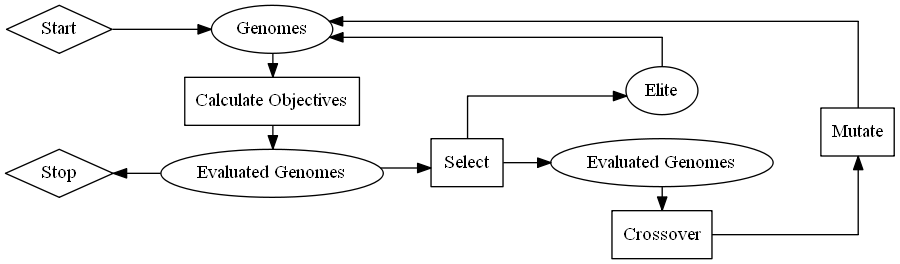
\includegraphics[width=\textwidth]{GA}
        \caption{``Life Cycle" of A Genetic Algorithm}\label{fig:GA}
    \end{figure}

    One note about figure \ref{fig:GA} is that the decision to go to the ``Stop"
    state is determined by some outside factor i.e. execution time. Otherwise
    it repeats infinitely - just like real life. Applying this generic algorithm to 
    our specific problem. We simply need to
    define each state in this diagram in the context of our problem.

    The \textit{Genomes} state for our problem is the set of \(f\)'s. Each gene is an
    \(f\) for a specific stock, but we have additional constraints, which is for 
    any genome \((f_1...f_m)\) made up of genes \(f_i\), the genome \textbf{must}
    abide by these laws:

    \begin{align*}
        \text{Law: } & \;
        0 < \left(
            \displaystyle\sum^{m}_{i=1} f_i
        \right) <= 1 \\
        \text{Law: } & \;
        \forall f_i \in (f_1...f_m) \to \left(
            0 < f_i <= 1
        \right) \\
    \end{align*}

    which more simply states, we can't bet more than our entire wealth over all the stocks or
    a negative bet. And on a single stock we can't place a negative bet more than our
    entire portfolio. \textbf{Note:} This is very different from how most genetic algorithms
    are implemented. They tend to be implemented as sequence of binary digits which makes
    mutation, and crossover easier. 

    The \textit{Select} state is a function which takes all pairs of evaluated genomes
    and their fitness. And based on how well each genome performs, will cull the
    list of genomes to a smaller list. This smaller list is the list of genomes
    which act as parents for the next generation.

    The \textit{Elite} state is another output from the select function, which is
    that the most fit genomes have their lifespan extended into the next generation.
    Importantly this elite population must be very small, as well as avoiding the
    chance for its genes to be destroyed by crossover and mutation. \cite{DeJong}
    This allows the best genome to always stay alive, and stops the GA from
    having to re-discover previously good results.

    The \textit{Crossover} state can simply be the same as any generic GA implementation,
    as we have no extra constraints to worry about. In the actual implementation
    a single point crossover, of high chance of occurrence was chosen. This was
    chosen arbitrarily, it could be worth a in-depth study to which crossover
    method would best perform for this specific problem. Since there is no catch all
    ``best" crossover method.

    The \textit{Mutate} state needs to make sure it follows the same constraints as
    genomes states has to follow. Furthermore since this step is after crossover,
    any genomes which violate the laws will be fixed in this step. Other than this,
    mutation can be any generic GA mutation. The specific mutation chosen was a
    simple Normal distributed mutation, which is randomly added or subtracted from
    the original gene. Similar to the specific crossover choice, this choice
    of mutation is probably worth its own in-depth study to optimize how fast
    the GA finds the solution. There is also no catch all ``best" mutation method.

    Finally the \textit{Calculate Objectives} state, which is the final product of all our
    mathematical exploration. Here we have two options the single variable option: equations
    \ref{eq:G}, \ref{eq:HPR_k}, and \ref{eq:Prob_k}. Or the decoupled multi-objective
    option: equations \ref{eq:DecoupleG} and \ref{eq:DecoupleR}.

    Other than the mathematical difference between single and multi-objective,
    another key difference between single objective and multi-objective is that for a
    nontrivial problem such as ours, no single solution exists that simultaneously
    optimizes each objective. This case of conflicting objectives means there is
    a (possibly infinite) number of Pareto optimal solutions, forming a Pareto front.
    The problem of sorting a set of genomes is complex problem, and furthermore
    does not remove problem of fronts forming rather than complete solutions.
    The way the results of our GA are sorted are according to the paper headed by
    Kalyanmoy Deb \cite{DebPratapAgarwalMeyarivan} in which they propose the
    NSGA-II, the cutting edge of multi-objective solution finding. This actually
    has a direct impact on the selection step of the GA.

\subsection{NSGA-II vs Other Multi-Objective Algorithms}

    As there exists multiple Pareto optimal solutions for our problem, what it means to ``solve"
    our problem, is not as simple as single objective problems. We actually want to create the
    Pareto set of optimal solutions and then to form a single solution we have to choose one of
    the Pareto solutions from that set.

    There are two methodologies to go about this selection of a single solution. A \textit{priori}
    methodology, in which the Pareto set is constrained by some rules provided by a user.
    These rules result in a single solution being used each step of GA. The other
    methodology is the \textit{posteriori} methodology, in which
    the full set of Pareto optimal solutions is kept and a user must decide which individual
    solution is kept only after the GA has finished execution.

    Linear scalarizing \& Non-linear scalarizing are two a priori ways to solve this problem
    \cite{KaisaMarko, Moffaert}. Both of the cited papers give a range of linear and non-linear
    functions which can be used either with weightings by the user, or utility functions.
    To list a few: The simplest being a weighted average of all the objectives, from
    which a single objective if found. Another version is a single point is chosen
    in the answer space, then the distance to that point is calculated and used to
    determine how good a solution is. A lower distance will mean its a better solution
    \cite{Buchanan}.

    To use utility functions as scalarizing solvers, this utility function will take
    the resulting objectives and return and ordering of ranking. Upon which the highest
    ranked is considered the best solution. This requires the user to construct
    a function which accurately represents the interests of user. A simple way
    to do this is to ask the user to list the objectives in a lexicographical order.
    But in practice a utility function is very hard to create, and the simple
    lexicographical solution is not well suited to our needs, as it requires
    strictly preferable objectives.

    To name some a posteriori methods, there's Normal Boundary Intersection \cite{Indraneel},
    Normal Constraint \cite{Messac}, Directed Search Domain \cite{Tohid}, and NSGA-II
    \cite{DebPratapAgarwalMeyarivan}. All except NSGA-II work by constructing several
    scalarizations, with each scalarization creating a Pareto optimal solution.
    This also leads those algorithms to end up in local maximum far to often and
    don't get the full efficient frontier.

    However NSGA-2 is different to the previous ones, and for the reason to be explained,
    and because its specifically useful for our problem, this is the algorithm that
    we use to find the Pareto frontier. To explain NSGA-2, first we need to explain
    NSGA, and non-domination.

    \textbf{Domination}: A solution \(x\) is said to dominate another solution \(y\) if:

    \begin{align*}
        & x \text{ is no worse than } y \text{ for all objectives} \\
        & x \text{ is strictly better than } y \text{ in at least one objective} \\
    \end{align*}

    This is denoted in most papers as \(x \prec y\), to further this: Among a set of solutions \(P\)
    the non-dominated sub set \(P'\) are those that are not dominated by any member of
    set \(P\). To follow on from this the a non-dominated set of the multi-objective search
    space, will be the global Pareto optimal set.

    NSGA-II has the following procedure: perform a non-dominated sorting in the population
    and classify them by front. i.e. sorted according ascending level of non-domination.

    \begin{figure}[H]
        \centering
        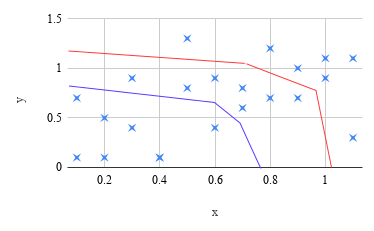
\includegraphics[width=.6\textwidth]{NSGArank}
        \caption{An example of non-dominated ranking}\label{fig:NSGArank}
    \end{figure}
    From this example graph (figure \ref{fig:NSGArank}), we have split the data up into 3 sets
    which are non-dominated
    by each other. The set contained by the blue and first line is a non-dominated sub set
    of the set between the two lines. The set between the two lines is also a non-dominated
    sub set of the final set. This allows us to assign a rank to each band.

    The next step is to make the next generation of parents from the front ranking
    set, as well as some random amount of the inferior bands. This population
    then goes under the next steps of the GA and the cycle is repeated.

    This method of multi-objective has some big advantages compared to the other methods,
    the most important being that the pareto set is collected instead by using the non-dominated
    sorting. While the solutions aren't guaranteed to be optimal pareto solutions, they
    get very close. Furthermore this method was designed with GA's in mind and therefore is
    optimized for this usage. Hence why I'm choosing to use NSGA-II in my solution.


\section{Implementation Details \& The Experiment}

    Now that we have a problem, and a method to solve it, all thats left is to actually
    implement it, and then test it on some data, comparing our hypothesis to the results.
    I chose to implement the system using Haskell. This is definitely a personal
    choice, for the standard reasons: familiarity, ease of use, having the environments
    set-up, and the strong type system. When working with a lot of ``pure"
    functions, as we would have to for this project. The implementation 
    of the mathematical part of this project was made significantly
    easier, less buggy, and probably more performant because of the language choice
    \footnote{Being pure makes parallelism a no cost feature \cite{HarrisMarlowJones, Chakravarty},
    which will give great performance improvements due to lightweight nature of the 
    computation, while needing lots of locking. }.
    In my eyes the mathematical functions
    being implemented purely reduces the chance to almost zero for there to be a translation
    error. This was helpful during the development, as any erroneous values implied a mistake
    in the maths.

    Another key choice made, was the use of Moo - a GA library \cite{Moo}. This came with all
    the normal advantages and disadvantages of using a library, time saved, tested by others, etc.
    It still required a fairly large amount of work to correctly integrate the
    problem into the library. Additionally you do not have complete control over the code,
    so any ``mistakes" or differences in behaviour are out of your control. However,
    this meant that once this work was done the actual execution of the GA was more simple.

    The experiment involved the following method. First I choose a portfolio I want to
    analyze, in this case I used the data set provided by my supervisor \cite{Dataset}.
    Obviously there are drawbacks to this as later explained in the results. The next step is
    to have some point of comparison, the obvious choice is to compare the GA to
    a completely naive spread i.e. evenly spread out the starting money over each stock.
    I also choose to compare the GA to the UK national interest rate \cite{BankOfE} to give an
    indication of how well the algorithm is performing compared to doing ``nothing". Another
    easy test to compare to is the idea of a portfolio putting all its eggs into one basket.
    Simply chose the best stock in terms of value increase, and your portfolio is simply that
    stock.

\subsection{Implementation Overview}

    The implementation is broken up into four main sections:

    \begin{itemize}
        \item{Dataset Parsing}
        \item{Calculating Correlations \& Risk}
        \item{Calculating Objectives}
        \item{Executing the GA}
    \end{itemize}

    \textit{Dataset Parsing} was implemented in a concrete form to directly work with the
    dataset I will use in the experiment. This means the code reads the CSV files,
    performs the necessary processing to convert them into the Haskell types, and then
    basic statistical analysis to extract trades.

    \textit{Calculating Correlations} is the implementation of the equation \ref{eq:Correlation}.
    Additionally we need to correlate every stock to every other stock. Because equation
    \ref{eq:DecoupleR} requires every stock included in the risk calculation has some value of
    correlation for all other stocks.

    Therefore in the worst case we need to do \(m!\) correlation calculations, each one requiring a
    full traversal of all the trades in the stock. This gives a full time complexity of 
    \(\bigO (nm!) \). This can be speed up a little bit in the actual implementation, firstly
    equation \ref{eq:Correlation} can be done in a single pass instead of two. Secondly we can
    half the number of permutations we need to do the correlation calculation for. Since we know
    correlation is symmetric, i.e. if the correlation of \(C_{x,y} = z\) then the correlation
    of \(C_{y,x}\) also equals \(z\). While this doesn't change the time complexity, it still helps
    the execution time, as we only need half as many calculations. On top of this, and as explained
    earlier, this correlation calculation can be run in parallel using the pure nature of the function.
    All of equation \ref{eq:Correlation} is done in a unique threads using Haskell to abstract away
    the thread management.

    Furthermore, we can calculate the correlations ahead of the GA execution so this only needs to be
    executed once and the results are stored in a hash map. In the implementation the results are
    retrieved
    with a slightly modified look up function, which when given a key of a pair of stocks, it will
    search for both permutations of either stock. This is because only one of the stocks is input to the
    table with the corresponding correlation, this reduces the size of the table, while the retrieval time
    remains essentially constant.

    \textit{Calculating Risk} is the implementation of the inner equation \ref{eq:DecoupleR} 
    i.e. (\(\forall y \in m \to P(k|y)\)). This equation
    requires the correlation list to be calculated, because of equation \ref{eq:Correlation} being a
    part of equation \ref{eq:DecoupleR}. It can also be optimized such that the individual
    probabilities of each stock (calculated by equation \ref{eq:StockProb}) are only needed to be
    calculated once.

    \textit{Calculating Objectives} is the implementation of equation \ref{eq:DecoupleG} and the complete
    implementation of equation \ref{eq:DecoupleR} using the earlier risk calculation, these
    equations both take a list of \(f\)'s as their input to be able to calculate \(G\) and \(R\).
    And once again, this implementation takes advantage of Haskell's low cost parallelism to speed
    up execution.

    \textit{Executing the GA}, as explained earlier the Moo GA Library \cite{Moo} was used in
    the implementation. The additional details added in my solution are the printing of the results,
    the constraints specified by the laws of a portfolio, and the actual programming interface
    between the equations and the library code.

\subsection{Testing Method}\label{section:TestingMethod}

    The general testing method was as follows. Over the dataset, split it into moving windows
    where each window covers a certain time range of data. The windowing is done to emulate
    the process of eventually considering that old enough data will become less useful
    as an indicator of future events. The only piece of data that will be kept regardless
    of window size, is the \(BL\). This is to be more realistic about the worst case scenario.
    As it could be seen as reasonable to say the \(BL\) of any asset is \(\infty\), if
    the value of the asset becomes unsellable, this rather extreme view however essentially means all
    algorithms would tell you to bet nothing, since thats the superior strategy. Instead
    this approach, takes into account the worst \(BL\) of any one stock over its lifetime.
    Since almost every asset has the potential to fall as far as it once did. Even if we only
    consider its most recent results in the window, it is helpful to suspect an asset could
    do that poorly again.

    The next step is to choose the window size and the dataset of assets to be tested upon.
    In my case I used my supervisor's dataset \cite{Dataset} and I elected to choose a window
    size of 3 years.

    After the window size and dataset is chosen the next stage is to run preliminary tests with
    differing lengths of time to find the a reasonable amount of time to run the GA based on
    the hardware. From that you have make a human decision to compromise the amount of time
    you allow the GA to find a solution and how much time you actually have to test the GA.

    Next, you actually run the GA from the start of your dataset over every window and record
    the results. All thats left would be to compare these results the naive spread of the
    portfolio, or any other investment strategy for that matter.

    The actual evaluation I am going to use is forward testing the portfolio. This means that
    the fractional amounts to put on each stock are ``placed" on those stocks. Then you
    calculate how much money would be made over the next year with those fractions. This test
    is good because the Portfolio will be tested against data it hasn't been trained on.
    So a window size of 3 would mean you need data from 4 years i.e. a window of 2000 to 2003
    would be tested on how much money it would make in 2004.

\subsection{Results}

    First the preliminary results of running the GA over 1 window (of 3 years) with different
    times to determine how much time to spend. It is also useful as this graph also shows
    the full pareto frontier.

    \begin{figure}[H] % fig:HowTheParetoFrontierChangesWithGADuration_2017-1Window
        % \centering
        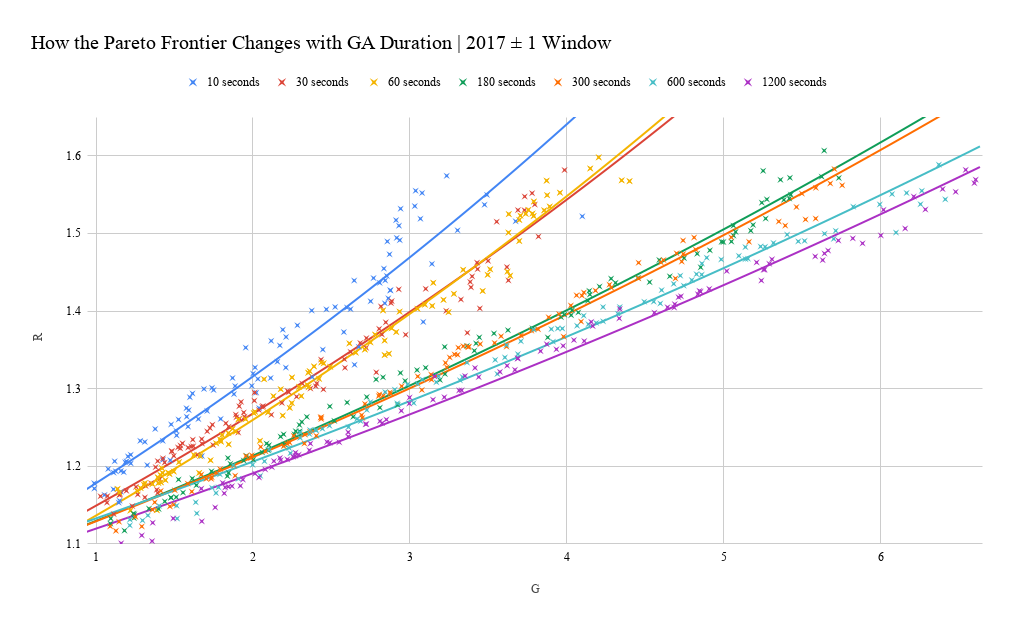
\includegraphics[width=\textwidth]{HowTheParetoFrontierChangesWithGADuration_2017-1Window}
        \caption{Preliminary : Pareto Frontier}
            \label{fig:HowTheParetoFrontierChangesWithGADuration_2017-1Window}
    \end{figure}

    The biggest takeaway from this graph is that it was very hard to improve \(R\) beyond
    the initial solutions, but the gain seemed to constantly improve given exponentially
    more time. There was a significant jump in results from 1 minute to 3 minutes,
    therefore I chose to do all future tests with 3 minutes. Once again this is slightly
    arbitrary, since if wanted the ``best" results I would've chosen 20 minutes (1200 seconds).
    But that amount of time for a single run is a bit extreme. Furthermore the sample size for
    each duration is only 1, so 3 minutes was more a estimated timing based loosely
    on this result.

    The next step was to run the GA and actually compare the results to other methods.
    The comparisons I have chosen are: A naive spread, which splits up its initial wealth
    evenly over every stock; a litmus test method, which simply takes the ``best" performing
    stock from the window, and puts all its wealth on that stock; and finally
    comparing it to putting you money in a bank offering UK national interest rates
    \cite{BankOfE}.

    For verification, by attempting to ensure the results aren't an anomaly, the GA was run 10
    times for each window. This is to help determine how consistent the GA is at producing
    similar performing portfolios and to compare how diverse the actual allocation
    of the stocks is. It was also run over many windows, to get more information
    on how different economic climates affect the performance. Finally, from the pareto
    set of portfolios produced by the GA, only 3 are chosen. It could have been worth
    it to test all of the portfolios produced by the GA but since you can only
    chose a single portfolio from the set, its realistically unfeasible to expect a
    test of all the portfolios. Since a human should make a choice about how much
    they prefer \(G\) (gain) or \(R\) (risk) and then choose a portfolio which most
    aligns with their preferred values. To emulate this human I will chose 3
    portfolios to test, representing 3 different peoples decision making; a risk
    averse person, a risk neutral person, and a risk sensitive person. Obviously
    this is a simplification of decision making, however, some method of choosing
    test portfolios is needed.

    To do this, the pareto set is sorted lexicographically, with the \(G\) and \(R\)
    values for the comparison method, where \(R\) was minimized. I then elected to choose,
    the first element from this set, the middle element, and the last element.
    These 3 portfolios were then carried forward and tested. From here on out
    these 3 portfolios are referred to as Highest \(G\) (the first element),
    the Median \(G/R\) (the middle element), and the Lowest \(R\) (the last element).
    Hence representing the 3 different people.

    \begin{figure}[H] % fig:AComparisonOfPortfolios 
        % \centering
        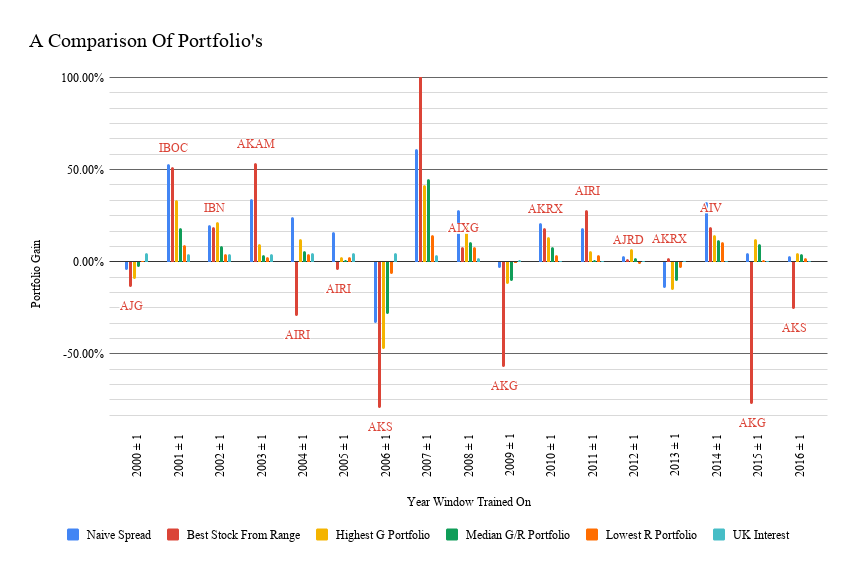
\includegraphics[width=\textwidth]{AComparisonOfPortfolios}
        \caption{Results from The Test. See appendix \ref{apd:AComparisonOfPortfoliosTable} for raw values}
            \label{fig:AComparisonOfPortfolios}
    \end{figure}

    Its evident from this graph that one result is missing and goes off the graph. This
    is the result from the 2007 window, and the appendix \ref{apd:AComparisonOfPortfoliosTable}
    shows the gain was 436.23\%. This result made the graph unreadable. Analyzing
    from these results we can see that the GA doesn't consistently outperform our basic
    tests. There are years which it is outperformed by either the best stock, or a naive
    spread, or UK interest. And there are years in which it outperforms those methods.
    Taking a closer
    look at one window, say 2004, we can see the prominence of the best stock method
    failing dramatically here, losing 29.71\% of the portfolios value. Whereas
    the portfolios chosen by the naive spread, risk averse, risk neutral, risk
    sensitive, and interest rate, all increase the value of the portfolio. However
    what's disappointing is that the best performing portfolio was simply the naive spread.
    Even the risk averse portfolio, only performs half as well as the naive spread.

    \begin{figure}[H] % fig:MeanAndVarianceOfPortfolioTypes
        % \centering
        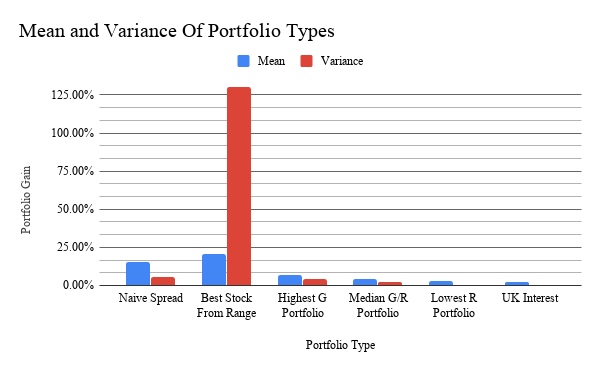
\includegraphics[width=\textwidth]{MeanAndVarianceOfPortfolioTypes}
        \caption{Measuring the Variance and Average Results from the different Methods. See \ref{apd:MeanAndVarianceOfPortfolioTypes} for raw results.}\label{fig:MeanAndVarianceOfPortfolioTypes}
    \end{figure}

    Averaging out all of the windows to try and get a better picture how it generally
    performs is done in figure \ref{fig:MeanAndVarianceOfPortfolioTypes}. In this graph
    we can see that on average: the naive spread and the best stock actually performed
    better than any other option, this is disappointing for our algorithm.

    The variance of the portfolios produced by the GA are not only lower, meaning that
    when it loses, it losses far less money than the other portfolios. However, when the GA wins
    it also wins far less money than the other portfolios. This is a
    desirable trait for the algorithm to have. Furthermore the risk formulation
    actually appears to work. The portfolios which elected to have lower \(R\)
    had a lower variance and hence are less risky. The lowest risk portfolios
    had a 10\(\times\) improvement in risk compared to the median portfolios, and 20\(\times\)
    compared to the highest \(G\) portfolios. As you can also see from the graph the best
    stock method was incredibly variable. This is partly due to the outlier in the 2007
    window and also due to large losses in 2006 and 2015. The best stock method
    is much riskier, which explains its extremely high variance of 129.94\%.

    This also links into the graph drawn in appendix \ref{apd:PerformanceOfPortfolioTypes}
    which takes the best portfolio from each window, and counts the number of each.
    And as is evident from the graph, the portfolios produced by the GA, do not
    do very well. Highest \(G\) portfolios manage to win 4 times, but both
    Median \(G/R\) and Lowest \(R\) fail to win a single time. Furthermore 3
    times UK interest (a.k.a the doing nothing with your money strategy)
    also wins, which shows how every method is still not consistent enough to
    be risk free.

    For completeness I also plotted the actual portfolios created by the GA, as this
    would indicate if the GA was over fitting or finding local maximums. These can
    be found in the appendix at \ref{apd:HighestGPortfolioDistributions},
    \ref{apd:MedianGRPortfolioDistributions}, and
    \ref{apd:LowestRPortolioDistributions}. The obvious takeaway from these is that
    emergent property of less variance can be explained by the GA's ``choice" to
    simply not invest when minimizing \(R\). Humorously the fact that this is emergent
    is a simple fact that you risk less, by playing less. Which is good that the GA
    ``discovered" this property, but also against the spirit of what portfolio
    optimization aims to achieve. It may be worth testing with the additional
    constraint on the GA to ensure it always spends all the portfolio. The Medain
    \(G/R\) portfolios allocates around 75\% of a portfolio,
    and the Lowest \(R\) allocates around 50\% of all the initial wealth!

    Another key distinction when comparing the three graphs is that the change in
    portfolio distribution over time windows is vastly different. The Highest
    \(G\) graph, \ref{apd:HighestGPortfolioDistributions}, show large amounts
    of variation year on year. Which looks like an attempt to adapt the portfolio
    to best stocks at the cost of riskier gains. Whereas the Lowest \(R\) graph
    shows good consistency across the years. This is very intriguing as the
    GA was still run on the exact same data, i.e. both only had 3 years of data to
    analyze. Yet the Lowest \(R\) portfolios tended to still choose the same stocks,
    with only minor variation each window.

    Finally one other measure to evaluate the algorithm is how consistent the portfolios
    are when run on the same data. Since we ran 10 tests on each window, we have a reasonable
    sample size to check with.

    \begin{figure}[H] % fig:VarianceOfPortfoliosOverTests
        % \centering
        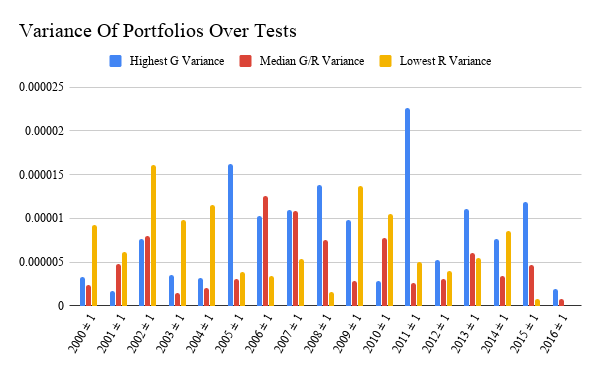
\includegraphics[width=\textwidth]{VarianceOfPortfoliosOverTests}
        \caption{The variance of the actual portfolios produced by the GA for each window}
            \label{fig:VarianceOfPortfoliosOverTests}
    \end{figure}

    Figure \ref{fig:VarianceOfPortfoliosOverTests} plots the average variance of the variances for
    each stock over the 10 tests. Another way to think about this metric is by taking the allocated
    portfolios from the 10 tests, then considering the value assigned by the 10 tests for 1 stock in
    particular; calculate the variance of those values from the 10 tests. Now do this for every stock and find the
    average of these variances. This value is then plotted to Figure
    \ref{fig:VarianceOfPortfoliosOverTests}. From this graph its important to note the scale of
    the y-axis, which is very small. The actual variance of the portfolios appears to be very
    good, if slightly random. Although this is expected of a genetic algorithm.

\section{Conclusion}

\subsection{How Well Has This Algorithm Performed?}

    Overall The performance leaves something to be desired. Figure
    \ref{fig:AComparisonOfPortfolios} and \ref{fig:MeanAndVarianceOfPortfolioTypes}
    shows how the actual performance was
    sub par compared to some very basic portfolios. The average value of a portfolio
    increased by 6.78\% using the highest gaining portfolios from the GA. This is lower
    than the best stock method (20.56\%) and naive spread (15.45\%). This shows
    that the GA doesn't actually achieve what we set out to do.

    Despite this the GA shows some good traits. Which is that choosing portfolios
    with a lower \(R\) value, actually correlates to less variance on the gain
    of a portfolio. This is promising, the actual amount the variance is reduced
    is significant. The highest risk portfolios were about 20 \(\times\) more
    variable than the lowest risk portfolios. Combined with the fact that the
    reduction in gain was only about 2 \(\times\) for this better
    variance. Thus showing that the risk correlation at least works with a mathematical
    interpretation.

\subsection{Evaluation Of The Implementation}

    I am confident that both algorithms described in section \ref{section:DecoupleG}
    are implemented bug-free over the set of assets used in testing. As explained
    the purity of Haskell makes me very confident that once the code compiled - and
    had matching types to that of the equations. Then it would be correct. A small
    set of manual tests were then executed on the equations, testing edge cases,
    and normal values. All of which passed.

    However this does not mean that it is actually implemented perfectly. Additional
    quick check tests \cite{QuickCheck} (Unit tests) could have been written to
    much more concretely say that every equation was fully implemented. This is
    one area that would need more work if algorithm was to have real world use.

    In terms of the genetic algorithm, the fact that I used a library \cite{Moo}
    which is already well tested. Made sure that the genetic part of the algorithm
    was implemented correctly. The only section which could do with additional
    quick check testing, is the constraints applied to the genes at each iteration
    of the genetic algorithm. Since this was a custom implementation tailored to
    this specific problem, it should also be tested throughly before this
    would be used in the real world.

\subsection{Evaluation of Testing Methods}

    In terms of testing on the single data set \cite{Dataset} I believe enough
    data was gathered to see how well the GA performed. Testing on different
    windows allows a look into how the algorithm would adapt to new data,
    say you used the algorithm to actually change your portfolio given a
    new year of data. Furthermore looking at figure \ref{fig:VarianceOfPortfoliosOverTests}
    the variance over the sets implies that each test run from the 10 tests was
    fairly similar. This leads to the belief that 10 tests was enough and more tests
    wouldn't have resulted in dramatically different portfolios, and therefore
    different gains.

    However more testing could be done, a data set which included more data from
    different markets with different assets. This would be another really good test
    to see if the GA just underperformed on this specific set of stocks. Or if its
    in fact flawed and always under performs on any market. A Bigger selection
    of assets is also worth testing against. As this dataset only had 28 individual
    stocks in it. Whereas it's completely normal to have 500 assets in a portfolio.

    Therefore I'd argue the actual testing done is conclusive about this set
    of stocks. But to get a full conclusive test on the GA itself would
    require the same test just with a much richer and broader data set as
    the basis for the test.

    Additionally this opens up the possibility of testing this GA with different
    correlation techniques. As described in section \ref{section:CalcR} there
    are many ways to calculate the correlation of stocks. And in this project,
    only one method is ever tested. The mathematical correlation of stocks. If the
    same tests were done with a different correlation method, and the results
    showed more promise. Then it would be safe to say that the correlation
    method would be superior if its results were better.

\pagebreak
\bibliographystyle{IEEEtran}
\bibliography{Report}
\pagebreak

\appendix

\section{Appendix: Results}

\subsection{A Comparison Of Portfolios Table}\label{apd:AComparisonOfPortfoliosTable}
    \begin{table}[H]
        \begin{tabular}
            {p{.09\textwidth}|p{.075\textwidth}|p{.075\textwidth}|p{.12\textwidth}|p{.12\textwidth}|p{.12\textwidth}|p{.12\textwidth}|p{.09\textwidth}}
            \bfseries Year Range & \bfseries Naive Spread & \bfseries Best Stock & \bfseries Best Stock From Range & \bfseries Highest G Portfolio & \bfseries Median G/R Portfolio & \bfseries Lowest R Portfolio & \bfseries UK Interest
            \csvreader[head to column names]{figures/AComparisonOfPortfoliosTable.csv}{}
            {\\\hline\csvcoli&\csvcolii&\csvcoliii&\csvcoliv&\csvcolv&\csvcolvi&\csvcolvii&\csvcolviii}
        \end{tabular}
    \end{table}

\subsection{Mean and Variance of Portfolio Types}\label{apd:MeanAndVarianceOfPortfolioTypes}
    \begin{table}[H]
        \begin{tabular}
            {p{.09\textwidth}|p{.09\textwidth}|p{.09\textwidth}|p{.13\textwidth}|p{.15\textwidth}|p{.13\textwidth}|p{.12\textwidth}}
            \bfseries - & \bfseries Naive Spread & \bfseries Best Stock & \bfseries Highest G Portfolio & \bfseries Median G/R Portfolio & \bfseries Lowest R Portfolio & \bfseries UK Interest
            \csvreader[head to column names]{figures/MeanAndVarianceOfPortfolioTypes.csv}{}
            {\\\hline\csvcoli&\csvcolii&\csvcoliii&\csvcoliv&\csvcolv&\csvcolvi&\csvcolvii}
        \end{tabular}
    \end{table}

\subsection{Performance Of Portfolio Types}\label{apd:PerformanceOfPortfolioTypes}
    \begin{figure}[H]
        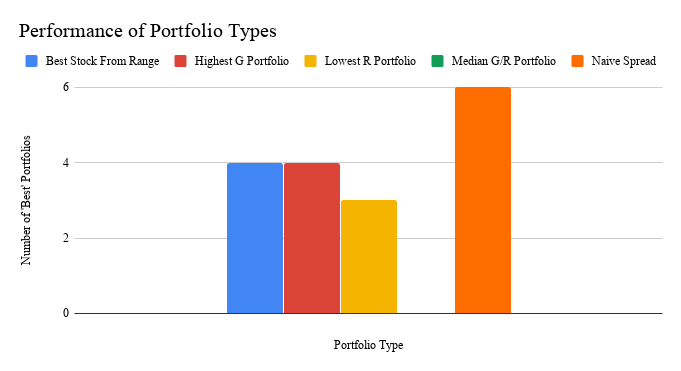
\includegraphics[width=\textwidth]{PerformanceOfPortfolioTypes}
    \end{figure}

\subsection{Highest \(G\) Portfolio Distributions}\label{apd:HighestGPortfolioDistributions}
    \begin{figure}[H]
        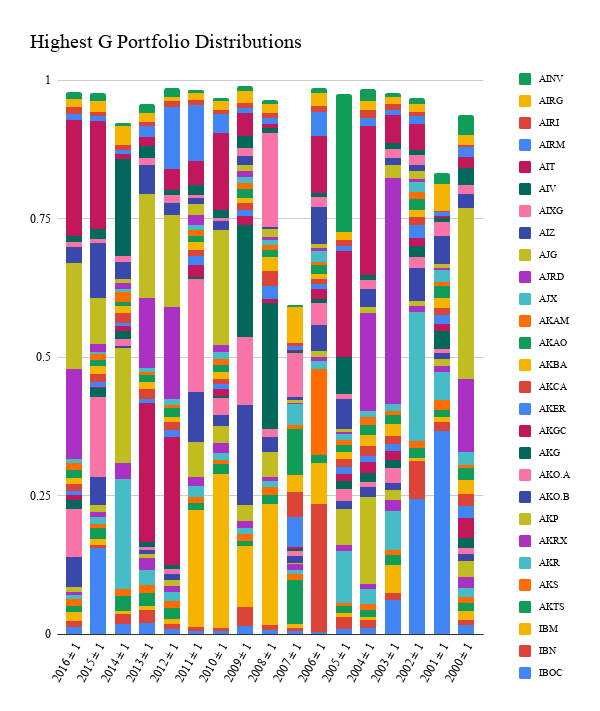
\includegraphics[width=\textwidth]{HighestGPortfolioDistributions}
    \end{figure}

\subsection{Median \(G/R\) Portfolio Distributions}\label{apd:MedianGRPortfolioDistributions}
    \begin{figure}[H]
        % \centering
        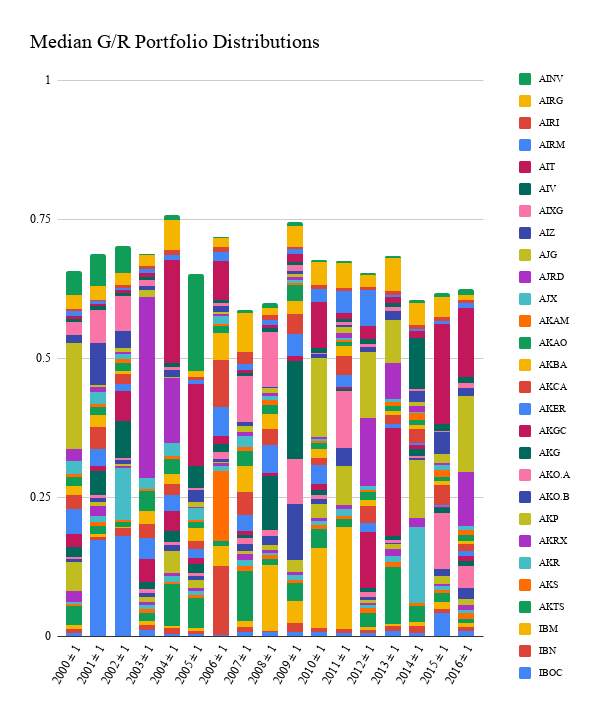
\includegraphics[width=\textwidth]{MedianGRPortfolioDistributions}
    \end{figure}

\subsection{Lowest \(R\) Portfolio Distributions}\label{apd:LowestRPortolioDistributions}
    \begin{figure}[H]
        % \centering
        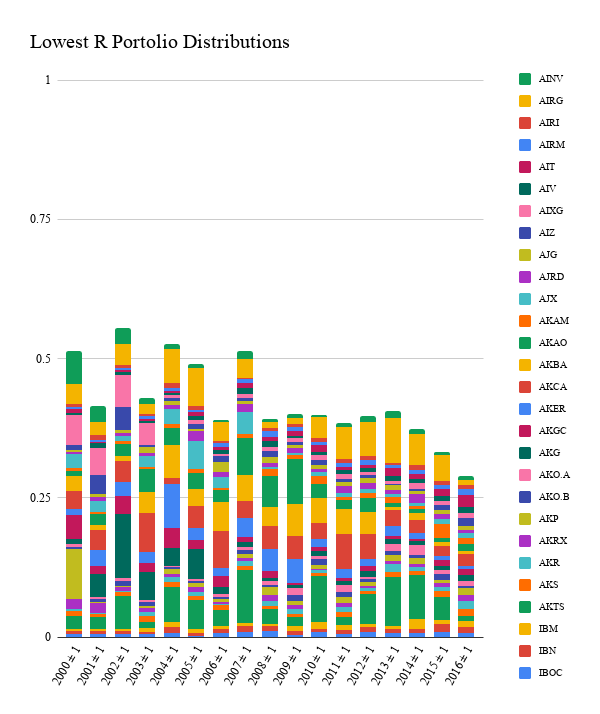
\includegraphics[width=\textwidth]{LowestRPortolioDistributions}
    \end{figure}

\end{document}
